\documentclass[12pt]{article}
%\usepackage[utf8]{inputenc}
%\documentclass[UTF8]{ctexart}
%\usepackage[UTF8, heading = false, scheme = plain]{ctex}
\usepackage{geometry}
%geometry{a4paper,scale=0.9}
\geometry{a4paper,left=1cm,right=1cm,top=1cm,bottom=2cm}
\usepackage{amsfonts}
\usepackage{color}
\usepackage{url}
%\usepackage{biblatex}
\usepackage{amsmath}
\usepackage{amssymb}
\usepackage{latexsym}
\usepackage[linesnumbered,ruled,lined]{algorithm2e}
\usepackage{pythonhighlight}
\usepackage{listings}
\usepackage{cite}
%\addbibresource{ref.bib}
%\bibliography{ref.bib}
\usepackage{caption}
\usepackage{graphicx, subfig}
\usepackage{float}
%\usepackage[fontset=ubuntu]{ctex}
%\usepackage{fontspec}
\usepackage{xeCJK}
%\usepackage[colorlinks,
%anchorcolor=black,
%citecolor=black]{hyperref}
%\setmainfont{SimSun}
\usepackage[section]{placeins}
\usepackage{enumitem}
\usepackage{framed}
\usepackage[framemethod=TikZ]{mdframed}
\usepackage{indentfirst}
\usepackage{setspace}%使用间距宏包
\linespread{1.5}

\lstset{
keywordstyle=\color{blue!70}\bfseries, %设置关键词为蓝色,需要引xcolor宏包,
basicstyle=\ttfamily, 
commentstyle=\ttfamily, %基本和注释的字体都使用默认的等宽,而非texlive调用的中文字体
%commentstyle=\color{red!50!green!50!blue!50},
showstringspaces=false, %不显示中间的空格
frame=shadowbox,  %边框
breaklines,%自动换行
columns=flexible,%不随便添加空格,只在已经有空格的地方添加空格,
%如果想要添加空格使用fixed作为参数(这是默认的),如果坚决不添加空格使用fullflexible作为参数.
frame=shadowbox, 
rulesepcolor=\color{red!20!green!20!blue!20}
}

\title{基于 TensorFlow 深入学习各类模型\cite{TensorFlow_Tutorial_Quick_Detailed}}
\author{leolinuxer}
%\date{June 2020}

\begin{document}
%\setlength{\parindent}{0pt}
\maketitle
\tableofcontents

\section{简单线性回归}
\subsection{数学表达式}
$$
\hat{y} = \beta_0 + \beta_1 x
$$

$\mu$ 代表误差;

线性回归的损失函数为残差平方和,即SSE(Sum of Squares for Error),在机器学习中它是回归问题中最常用的损失函数:
$$
L = \sum_{i=1}^n(y_i - \hat{y}_i)^2 = \sum_{i=1}^n\Big(y_i - (\hat{\beta}_0 + \hat{\beta}_1x_i)\Big)^2
$$

\subsection{求解方法——最小二乘法}
$$
\frac{\partial L}{\partial \beta_0} = 2\sum_{i=1}^n(y_i - \hat{\beta}_0 - \hat{\beta}_1 x_i) = 0
$$
$$
\frac{\partial L}{\partial \beta_1} = 2\sum_{i=1}^n(y_i - \hat{\beta}_0 - \hat{\beta}_1 x_i) x_i = 0
$$

\subsection{TF 实现}
代码地址:\url{codes/learn/tf_simple_linear_regression.py}
\begin{python}
#import tensorflow as tf
import tensorflow.compat.v1 as tf
tf.disable_v2_behavior()
import numpy as np
import matplotlib.pyplot as plt

#定义一个函数来归一化输入数据
def normalize(X):
    mean = np.mean(X)
    std = np.std(X)
    X = (X - mean) / std
    return X

def train():
    #使用 TensorFlow contrib 数据集加载波士顿房价数据集,并将其分解为 X_train 和 Y_train。可以对数据进行归一化处理:
    # default save path: ~/.keras/datasets/boston_housing.npz
    boston = tf.keras.datasets.boston_housing.load_data()
    boston_data = boston[0]
    X_train, Y_train = boston_data
    #选择第6维特征:RM (average number of rooms per dwelling)
    X_train = X_train[:, 5]
    X_train = normalize(X_train)
    n_samples = X_train.shape[0]

    #为训练数据声明 TensorFlow 占位符:
    X = tf.placeholder(tf.float32, name = 'X')
    Y = tf.placeholder(tf.float32, name = 'Y')

    #创建 TensorFlow 的权重和偏置变量且初始值为零
    w = tf.Variable(0.0, name = 'weight')
    b = tf.Variable(0.0, name = 'bias')

    #定义用于预测的线性回归模型和损失函数
    Y_hat = X * w + b
    #Y_hat = tf.tensordot(X, w, axes=1) + b
    loss = tf.square(Y - Y_hat, name = 'loss')

    #选择梯度下降优化器
    #optimizer = tf.train.GradientDescentOptimizer(learning_rate = 0.01, name='GradientDescentOptimizer').minimize(loss)
    optimizer = tf.train.AdamOptimizer().minimize(loss)
    #optimizer = tf.train.MomentumOptimizer(learning_rate=0.05, momentum=0.9, use_nesterov=True).minimize(loss)

    #声明初始化操作符
    init_op = tf.global_variables_initializer()
    total = []

    #现在,开始计算图,训练 100 次:
    with tf.Session() as sess:
        # Initialize variables
        sess.run(init_op)

        writer = tf.summary.FileWriter('graphs', sess.graph)

        #Train the model for 100 times
        for i in range(100):
            total_loss = 0
            for x, y in zip(X_train, Y_train):
                _, l = sess.run([optimizer, loss], feed_dict = {X:x, Y:y})
                total_loss += l
            total.append(total_loss / n_samples)
            print('Epoch {0}: Loss {1}'.format(i, total_loss/n_samples))
        writer.close()
        b_value, w_value = sess.run([b, w])

    #查看结果
    Y_pred = X_train * w_value + b_value
    print('Done')

    plt.plot(X_train, Y_train, 'bo', label = 'Real Data')
    plt.plot(X_train, Y_pred, 'r', label = 'Predicted Data')
    plt.legend()
    plt.show()
    plt.plot(total)
    plt.show()

if __name__ == '__main__':
    train()
\end{python}

从下图中可以看到,简单线性回归器试图拟合给定数据集的线性线:
\begin{figure}[H]
    \centering
    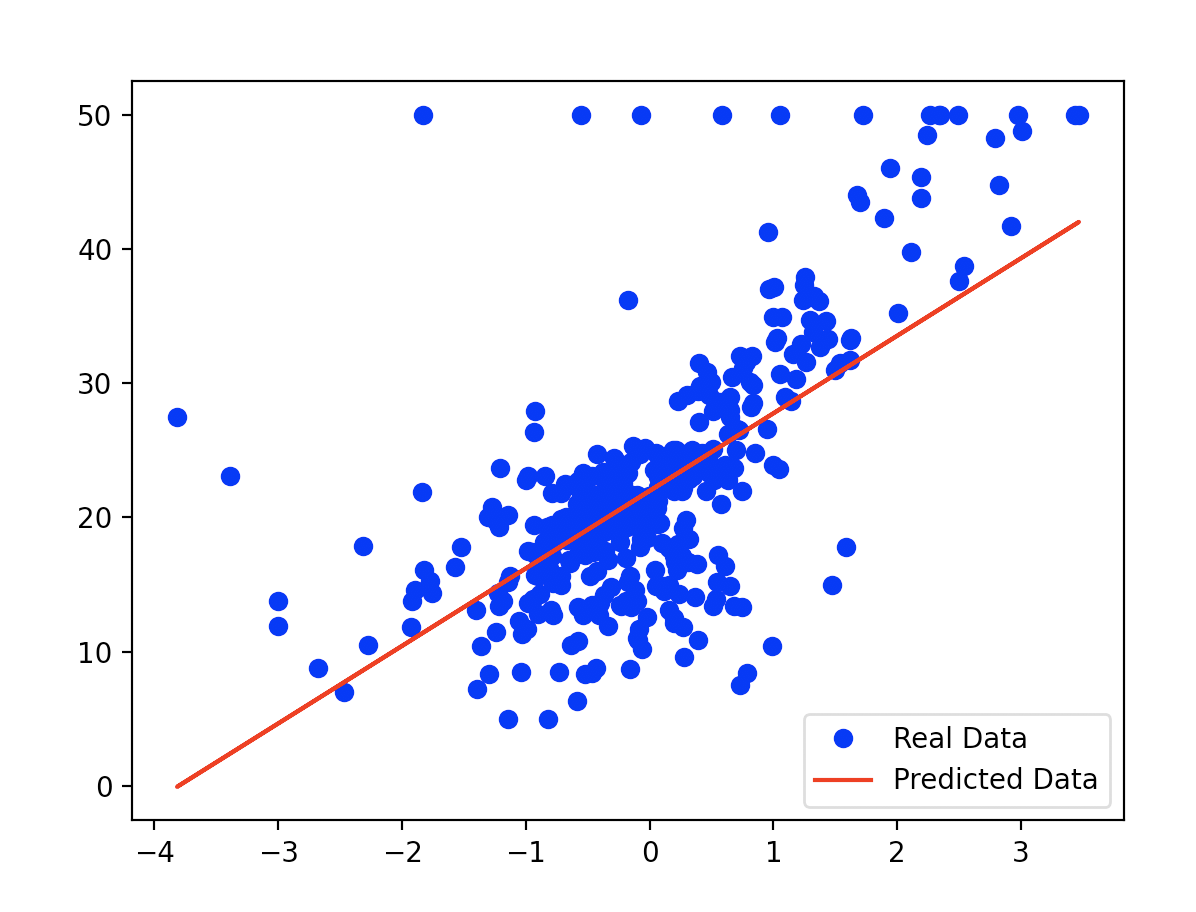
\includegraphics[width=.4\textwidth]{fig/codes/tf_simple_linear_regression_1.png}
\end{figure}

在下图中可以看到,随着模型不断学习数据,损失函数不断下降:
\begin{figure}[H]
    \centering
    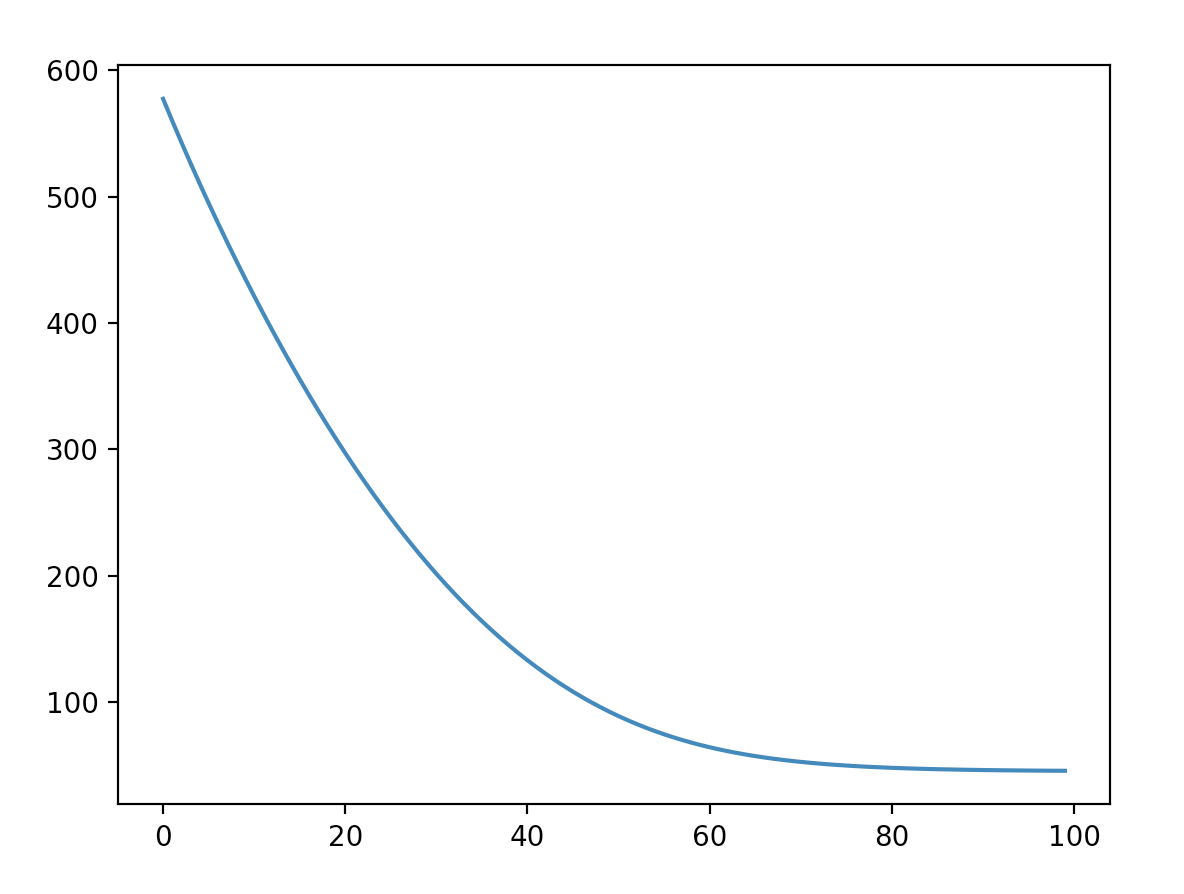
\includegraphics[width=.4\textwidth]{fig/codes/tf_simple_linear_regression_2.png}
\end{figure}

在终端执行
\begin{lstlisting}
tensorboard --logdir=graphs
\end{lstlisting}
在浏览器中打开,可以看到简单线性回归器的 TensorBoard 图:
\begin{figure}[H]
    \centering
    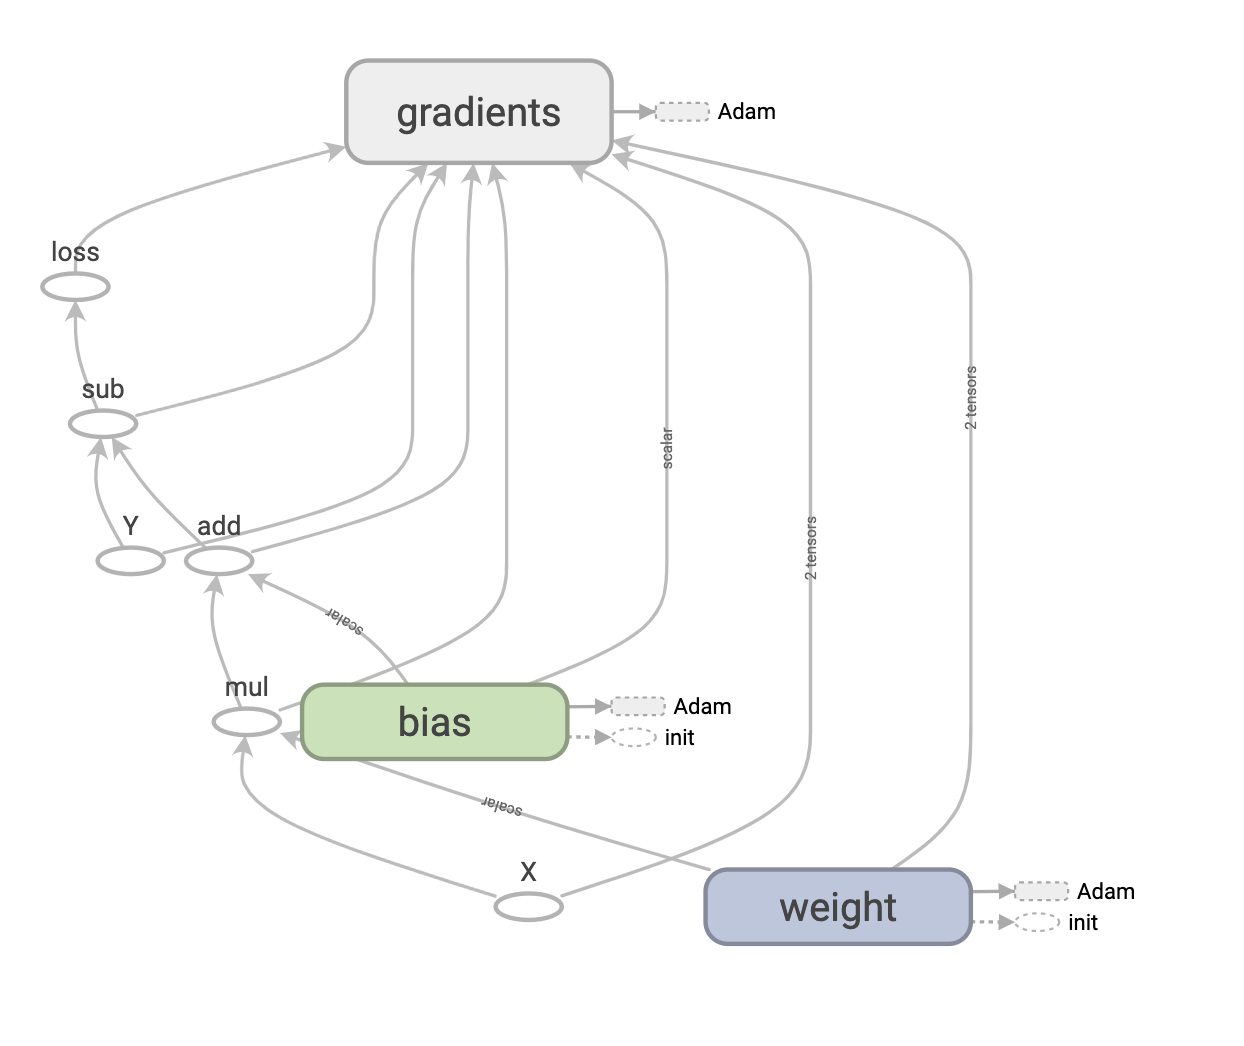
\includegraphics[width=.6\textwidth]{fig/codes/tf_simple_linear_regression_3.png}
\end{figure}

从图中可以清晰地看出前向计算过程:
\begin{align*}
& \hat{Y} = X \ mul \ weight \ add \ bias \\
& loss = Y \ sub \ \hat{Y} \\
\end{align*}

双击展开 gradient 节点,可以看到梯度的计算过程。可以看到它需要 7 个输入并使用 Adam 计算梯度,对权重和偏置进行更新
\begin{figure}[H]
    \centering
    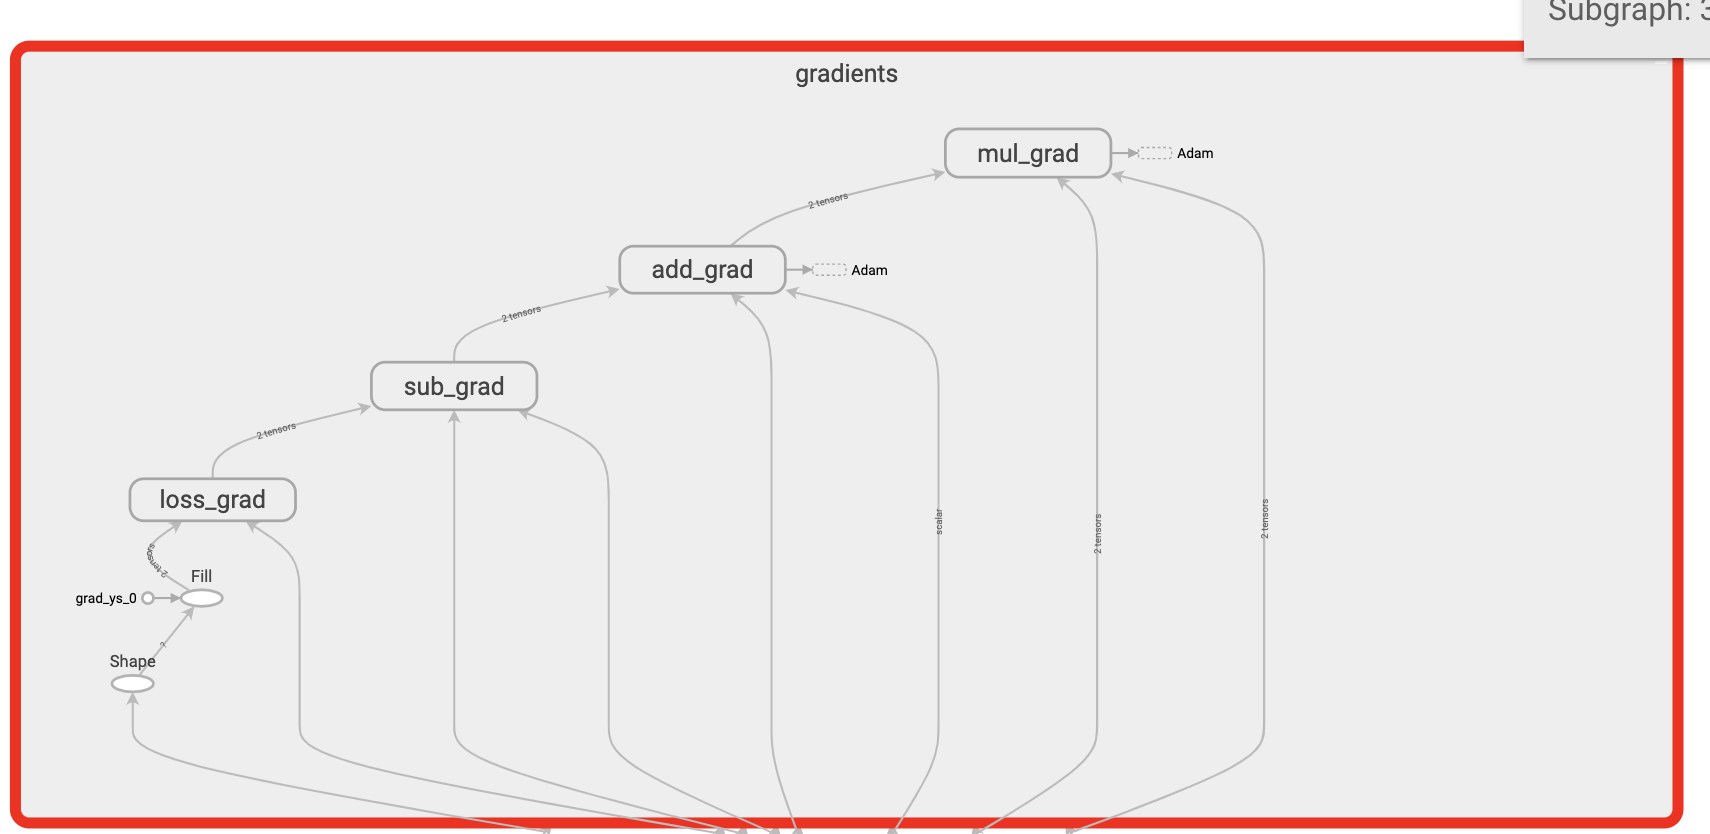
\includegraphics[width=1\textwidth]{fig/codes/tf_simple_linear_regression_4.png}
\end{figure}

\section{多元线性回归}
\subsection{TF 实现}
代码地址:\url{codes/learn/tf_multi_linear_regression.py}
\begin{python}
import os
import sys
#加入如下语句,应对错误:OMP: Error #15: Initializing libiomp5.dylib, but found libiomp5.dylib already initialized
os.environ['KMP_DUPLICATE_LIB_OK'] = 'TRUE'

……

#另外,这里添加一个额外的固定输入值将权重和偏置结合起来。为此定义函数 append_bias_reshape()。该技巧有时可有效简化编程
# print(X_train.shape, Y_train.shape)
# X_train, Y_train = append_bias_reshape(X_train, Y_train)
# print(X_train.shape, Y_train.shape)
# (404, 13) (404,)
# (404, 14) (404, 1)
def append_bias_reshape(features, labels):
    m = features.shape[0]
    n = features.shape[1]
    x = np.reshape(np.c_[np.ones(m), features], [m, n + 1])
    y = np.reshape(labels, [m, 1])
    return x, y
    
……

    m = len(X_train) # Number of training examples
    n = 13 + 1        # Number of features + bias
    #n = 12

    #为训练数据声明 TensorFlow 占位符:
    X = tf.placeholder(tf.float32, name = 'X', shape=[m,n])
    Y = tf.placeholder(tf.float32, name = 'Y')

    #创建 TensorFlow 的权重
    w = tf.Variable(tf.random_normal([n, 1]), name = 'weight')

    #定义用于预测的线性回归模型和损失函数
    Y_hat = tf.matmul(X, w)
    loss = tf.reduce_mean(tf.square(Y - Y_hat, name = 'loss')) + 0.6 * tf.nn.l2_loss(w)
    
……

    #现在,开始计算图,训练 100 次:
    with tf.Session() as sess:
        # Initialize variables
        sess.run(init_op)

        writer = tf.summary.FileWriter('graphs', sess.graph)

        #Train the model for 100 times
        for i in range(100):
            _, l = sess.run([optimizer, loss], feed_dict = {X:X_train, Y:Y_train})
            total.append(l)
            print('Epoch {0}: Loss {1}'.format(i, l))
        writer.close()
\end{python}
在下图中可以看到,随着模型不断学习数据,损失函数不断下降:
\begin{figure}[H]
    \centering
    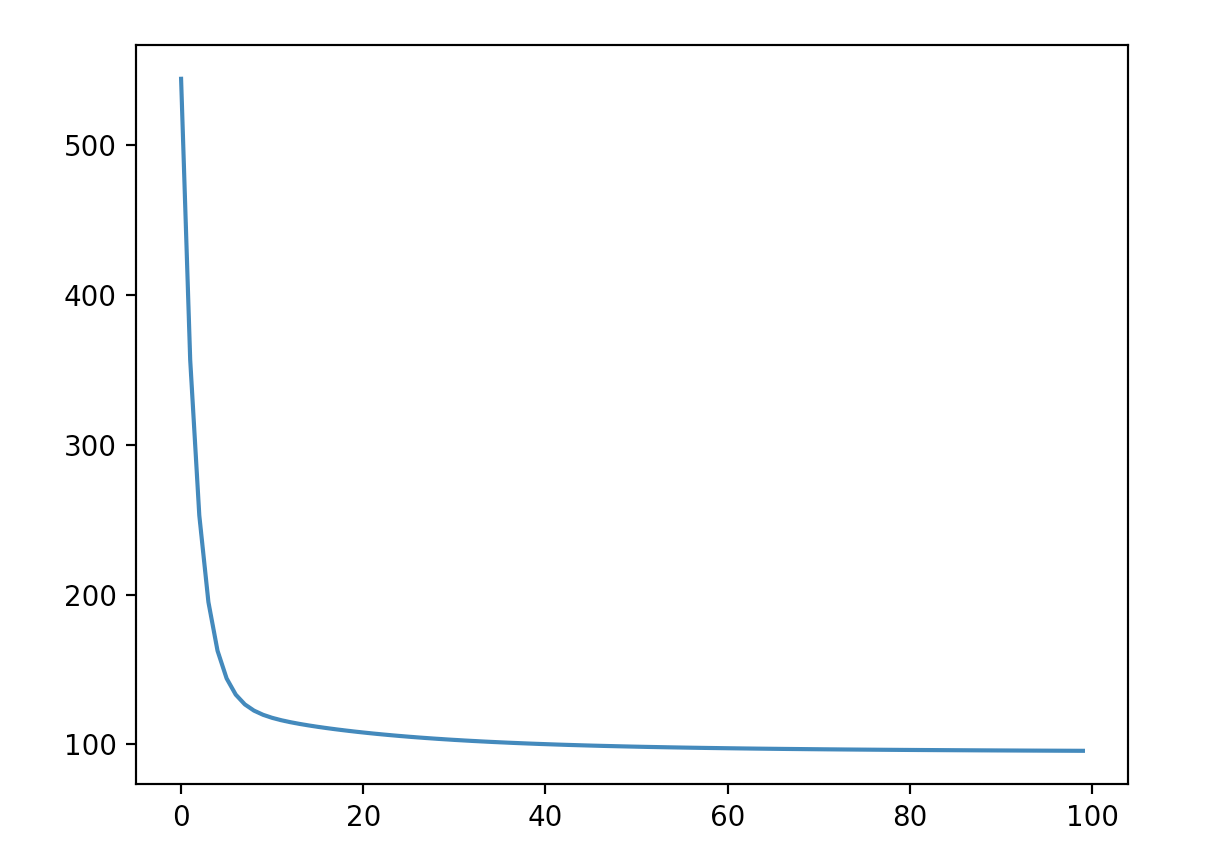
\includegraphics[width=.4\textwidth]{fig/codes/tf_multi_linear_regression_1.png}
\end{figure}

\section{TensorFlow逻辑回归处理MNIST数据集}

%\printbibliography
\bibliography{../ref}
\bibliographystyle{IEEEtran}
\end{document}